\documentclass[11pt]{article}

\usepackage{pablo-devoir}
\usepackage{pablo-listings}
\usepackage[a5paper,margin=1cm]{geometry}

\pagestyle{empty}

\title{Fonctions\\Corrigé}
\date{2/12/14}
\classe{2\up{des}14}
\dsnum{DS 3}

\begin{document}

\maketitle

\begin{exercice}[Images et antécédents --- 7 points]
  \emph{Répondre aux questions par lecture graphique.}
  \begin{enumerate}
    \item \emph{On considère la fonction $f$ représentée ci-dessous.}
      \begin{center}
        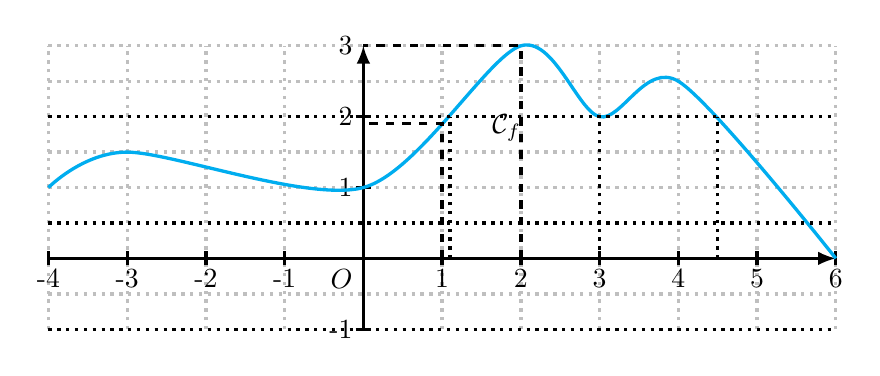
\begin{tikzpicture}[very thick,xscale=1, yscale=0.9]
          \draw[dotted, lightgray, xstep=1, ystep=.5] (-4, -1) grid (6, 3);
          \draw[-latex] (-4,0) -- (6,0);
          \draw[-latex] (0,-1) -- (0,3);
          \foreach \x in {-4, -3, -2, -1, 1, 2, 3, 4, 5, 6} {
            \draw (\x,0) node[below]{\x};
            \draw (\x,{0.1}) -- (\x,{-0.1});
          }
          \foreach \y in {-1, 1, 2} {
            \draw (0,\y) node[left]{\y};
            \draw (-.1, \y) -- (.1, \y);
          }
          \draw [cyan] plot [smooth, tension=0.5] coordinates {
            (-4,1)
            (-3, 1.5)
            (0, 1)
            (2, 3)
            (3, 2)
            (4, 2.5)
            (6, 0)
          };
          \draw (0,0) node[below left]{$O$};
          \draw (1.5, 1.5) node[above right]{$\mathcal{C}_f$};

      % Solutions
          \draw[dashed] (1,0) -- (1, 1.9) -- (0, 1.9);
          \draw[dashed] (2,0) -- (2, 3) -- (0, 3) node[left]{3};
          \draw[dotted] (-4, 2) -- (6,2);
          \draw[dotted] (1.1, 0) -- (1.1, 2);
          \draw[dotted] (3, 0) -- (3, 2);
          \draw[dotted] (4.5, 0) -- (4.5, 2);
          \draw[dotted] (-4, -1) -- (6, -1);
          \draw[dotted] (-4, .5) -- (6, .5);
        \end{tikzpicture}
      \end{center}
      \begin{enumerate}
        \item \emph{Déterminer $f(1)$.} $f(1)=1,9$
        \item \emph{Déterminer l'image de $2$ par $f$.} $f(2)=3$
        \item \emph{Quels sont le(s) antécédent(s) de $2$ par $f$ ?} Les antécédents sont $1,1$, $3$ et $4,5$.
        \item \emph{Résoudre graphiquement $f(x)=-1$.} Il n'y a pas de solutions.
        \item \emph{Déterminer un nombre $k$ tel que $f(x)=k$ ait une seule solution.} Par exemple, pour $k=0,5$, l'équation $f(x)=0,5$ n'a qu'une solution.
      \end{enumerate}
    \item \emph{Déterminer les solutions de $g(x)=h(x)$ (où les courbes de $g$ et $h$ sont représentées ci-dessous).}
      \begin{center}
        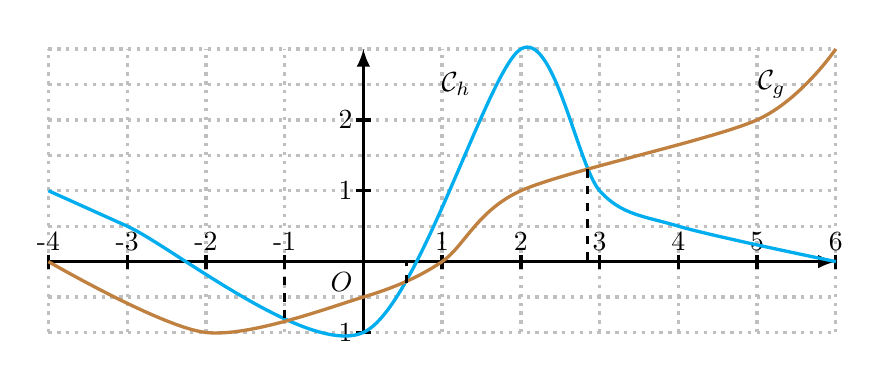
\begin{tikzpicture}[very thick,xscale=1, yscale=0.9]
          \draw[dotted, lightgray, xstep=1, ystep=.5] (-4, -1) grid (6, 3);
          \draw[-latex] (-4,0) -- (6,0);
          \draw[-latex] (0,-1) -- (0,3);
          \foreach \x in {-4, -3, -2, -1, 1, 2, 3, 4, 5, 6} {
            \draw (\x,0) node[above]{\x};
            \draw (\x,{0.1}) -- (\x,{-0.1});
          }
          \foreach \y in {-1, 1, 2} {
            \draw (0,\y) node[left]{\y};
            \draw (-.1, \y) -- (.1, \y);
          }
          \draw [cyan] plot [smooth, tension=0.5] coordinates {
            (-4,1)
            (-3, 0.5)
            (0, -1)
            (2, 3)
            (3, 1)
            (4, 0.5)
            (6, 0)
          };
          \draw [brown] plot [smooth, tension=0.5] coordinates {
            (-4,0)
            (-2, -1)
            (0, -.5)
            (1, 0)
            (2, 1)
            (5, 2)
            (6, 3)
          };
          \draw (0,0) node[below left]{$O$};
          \draw (1.5, 2.5) node[left]{$\mathcal{C}_h$};
          \draw (5.5, 2.5) node[left]{$\mathcal{C}_g$};

          % Solutions
          \draw[dashed] (-1, -.8) -- (-1, 0);
          \draw[dashed] (0.55, -.3) -- (.55, 0);
          \draw[dashed] (2.85, 1.3) -- (2.85, 0);
        \end{tikzpicture}
      \end{center}
      Les solutions sont les abscisses des points d'intersection des courbes de $g$ et $h$, c'est-à-dire : $-1$, $0,6$, $2,9$.
  \end{enumerate}

\end{exercice}

\begin{exercice}[Variations --- 4 points]
  Voici le tableau de variations d'une fonction $f$.

  \begin{center}
    \begin{tikzpicture}[xscale=1,yscale=1]
      \tkzTabInit[lgt=1,espcl=2]
      {$x$ /1,
        $f$ /2
      }
      {0, 2, 4, 5}%
      \tkzTabVar{-/1, +/2, -/1, +/4}
    \end{tikzpicture}
  \end{center}
  \begin{enumerate}
    \item \emph{Comparer $f(3)$ et $f(4)$.} On lit sur le tableau de variations que $f$ est décroissante entre 2 et 4. Or, $3<4$, donc $f(3)\geq f(4)$.
    \item \emph{Tracer la courbe d'une fonction $f$ pouvant correspondre à ce tableau.}
      \begin{center}
        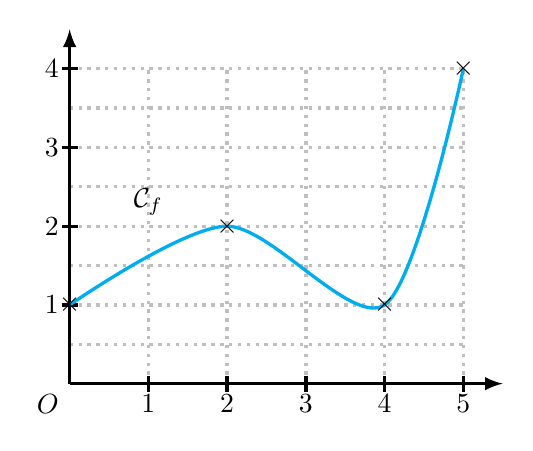
\begin{tikzpicture}[very thick,xscale=1, yscale=1]
          \draw[dotted, lightgray, xstep=1, ystep=.5] (0, 0) grid (5, 4);
          \draw[-latex] (0,0) -- (5.5,0);
          \draw[-latex] (0,0) -- (0,4.5);
          \foreach \x in {1, 2, ..., 5} {
            \draw (\x,0) node[below]{\x};
            \draw (\x,{0.1}) -- (\x,{-0.1});
          }
          \foreach \y in {1, 2, ..., 4} {
            \draw (0,\y) node[left]{\y};
            \draw (-.1, \y) -- (.1, \y);
          }
          \draw [cyan] plot [smooth, tension=0.5] coordinates {
            (0, 1)
            (2, 2)
            (4, 1)
            (5, 4)
          };
          \draw (0,0) node[below left]{$O$};
          \draw (1, 2) node[above]{$\mathcal{C}_f$};
          \foreach \point in {(0,1), (2,2), (4,1), (5,4)} {
            \draw \point node{$\times$};
          }
        \end{tikzpicture}
      \end{center}
  \end{enumerate}
\end{exercice}

\begin{exercice}[Algorithme --- 2 points]
  Dans un magasin, le tarif des photocopies est le suivant :
  \begin{itemize}[$\bullet$]
    \item Les vingt premières photocopies : 0,1~\euro{} pièce ;
    \item Les trente suivantes : 0,05~\euro{} pièce ;
    \item Toutes les autres : 0,01~\euro{} pièce.
  \end{itemize}
  \emph{
    Recopier sur votre copie l'algorithme suivant, et le compléter, pour qu'étant donné un nombre $n$, il affiche le prix de $n$ photocopies.
  }

  Commençons par étudier ce qui se passe pour différentes valeurs de $n$, avec des exemples.

  \begin{itemize}
    \item Supposons que j'achète 15 photocopies. C'est inférieur à 20, donc chacune me coûte 0,1~\euro, soit 1,5~\euro{} au total.
    \item Supposons maintenant que je fasse 45 photocopies. Les vingt premières coûtent toujours 0,1~\euro{}, et les 25 suivantes coûtent moins cher : 0,05~\euro.
    \item Enfin, pour 100 photocopies, les 20 premières coûtent $20\times0,1$~\euro{}, les 30 suivantes coûtent $30\times0,05$~\euro, et les 50 dernières coûtent $50\times0,01$~\euro.
  \end{itemize}

  Traduisons cela par un algorithme.

  \begin{lstlisting}[language=naturel,frame=lines,mathescape=true]
  Lire n
  Si $n\leq20$
  Alors
    Afficher 0,1 * n
  Sinon
    Si $n\leq50$
    Alors
      Afficher 0,1 * 20 + 0,05 * (n-20)
    Sinon
      Afficher 0,1 * 20 + 0,05 * 30 + 0,01 * (n-50)
  FinSi
  \end{lstlisting}
\end{exercice}

\begin{exercice}[Problème --- 7 points]
  Une fermière dispose de 100~m de cloture pour faire paître ses moutons. Elle souhaite faire une cloture rectangulaire qui ait la plus grande aire possible.

  \begin{center}
    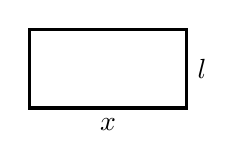
\begin{tikzpicture}[very thick]
      \draw (0,0) -- ++(2, 0) node[midway, below]{$x$} -- ++(0,1) node[midway, right]{$l$} --  ++(-2, 0) -- cycle;
    \end{tikzpicture}
  \end{center}
  On appelle $x$ et $l$ les longueurs des côtés en mètres.
  \begin{enumerate}
    \item 
      \begin{enumerate}
        \item \emph{Exprimer le périmètre en fonction de $x$ et $l$.} Le périmètre du rectangle est $2l+2x$.
        \item \emph{En déduire que $l=50-x$.} On sait que le périmètre de l'enclos est $100m$. Donc :
          \begin{align*}
            2l+2x&=100\\
            \frac{2l+2x}{2}&=\frac{100}{2}\\
            l+x&=50\\
            l&=50-x
          \end{align*}
      \end{enumerate}
    \item \emph{On appelle $\mathcal{A}(x)$ l'aire de l'enclos, en $m^2$, en fonction de $x$.}
      \begin{enumerate}
        \item \emph{Quel est le domaine de définition de $\mathcal{A}$ ?} La variable $x$ est une longueur, donc $x$ est supérieur à 0, et si $x$ est supérieur à 50, alors $l=50-x$ serait négatif, ce qui n'est pas possible (car $l$ aussi est une longueur). Bilan : le domaine de définition de $\mathcal{A}$ est $\left[ 0;50 \right]$.
        \item \emph{Montrer que $\mathcal{A}(x)=x\left( 50-x \right)$.} L'aire d'un rectangle est le produit de la longueur par la largeur, soit $\mathcal{A}(x)=l\times x$. Mais $l=50-x$, donc $\mathcal{A}(x)=\left( 50-x \right)x$.
      \end{enumerate}
    \item \emph{Le tableau de variations de $\mathcal{A}$ est le suivant.}
      \begin{center}
        \begin{tikzpicture}[xscale=1,yscale=1]
          \tkzTabInit[lgt=1,espcl=2]
          {$x$ /1,
            $\mathcal{A}$ /2
          }
          {0, 25, 50}%
          \tkzTabVar{-/0, +/625, -/0}
        \end{tikzpicture}
      \end{center}
      \emph{Quel est l'aire maximale que peut prendre l'enclos ? Quelle est alors la forme de l'enclos ?} On lit sur le tableau de variations que le maximum de la fonction est 625. Donc l'aire maximale de l'enclos est $625m^2$. Ce maximum est atteint pour $x=25$. Dans ce cas, $l=50-x=50-25=25$. Nous avons donc un rectangle de côtés 25 et 25 : c'est un carré.
    \item \emph{\emph{Bonus} Avec la même longueur de cloture, est-il possible de faire un enclos encore plus grand ?} Si la fermière dispose sa bordure en cercle et non pas en rectangle, elle peut faire en enclos encore plus grand.
  \end{enumerate}
\end{exercice}
\end{document}
